\Chapter{Numerical Experiment}
Option Pricing has always been a challenging topic in financial mathematics.
Here we are going to demonstrate several examples of pricing different options with ccontrol variates.

\Section{Asian Option}

There are two types of asian options, depends on which types of mean you want to use. For this example we take arithematic mean asian call option as our target function, whose payoff function is
\[ C_{T}^{Amean} = \max\Big(\frac{1}{d}\sum_{j=1}^{d}S(jT/d)-K, 0\Big)\]

\begin{table}[h]
    \centering
	\caption{Parameter Setup for Up and In Barrier Call Option}
	\begin{tabular}{lllllll}
		\hline\hline
        S0 & K & TimeVector & r & volatility & abstol & reltol \\[0.5ex]
        \hline
        120  & 130 & 1/52:1/52:16/52 & 0.01 & 0.5 & 1e-3 & 0\\[1ex] 
        \hline
	\end{tabular}
\end{table}

\begin{table}[h]
    \centering
	\caption{Results of cubSobol, cv\_old and cv\_new with Asian Option}
    \begin{tabular}{rrrrrr}  
    \hline\hline
	\multicolumn{3}{c}{Sample Size}
		&\multicolumn{3}{c}{Time Cost} \\
    \hline
	 cubSobol&cv\_old&cv\_new
    &cubSobol&cv\_old&cv\_new\\[0.5ex]
    \hline
		 65535&8192&9011
    &0.2783&0.1034&0.0673\\[1ex]
    \hline
	\end{tabular}
\end{table}

Figure ~\ref{fg:cvEX1} shows decrease rate the walsh coefficients for the target function and control variates in this example.

\begin{figure}[h]
    \centering
    %\setlength{\unitlength}{0.14in}     % selecting unit length
    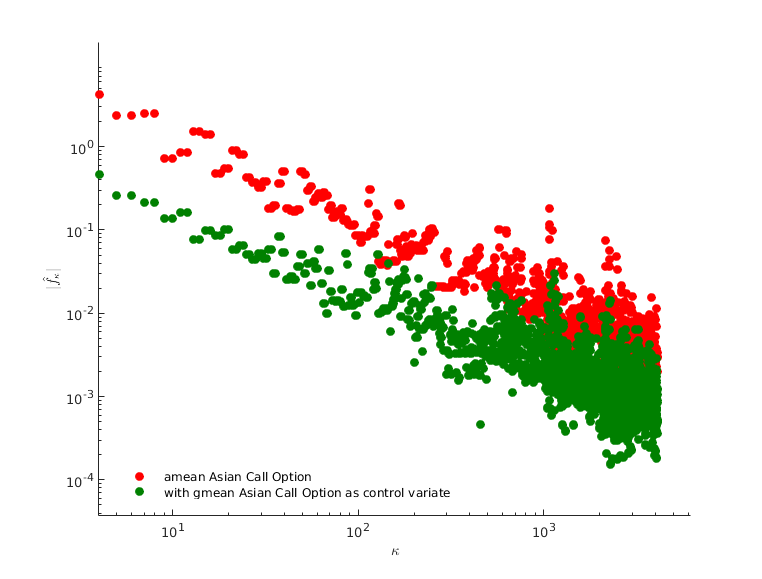
\includegraphics[width=0.8\textwidth]{figures/cvEx1.eps}
    \label{fg:cvEX1}
    \caption{Walsh coefficients of $f$}
\end{figure}

\Section{Barrier Option}

We will take up and in barrier call option as an example. Here is the payoff function for up and in barrier call option.
\[ C_{T}^{U\&I} = (S_T-K)^+1_{ \{\max S_t \geq Barrier\}} \]

From the payoff function it is naturally to consider european call option as control variates. Since if we take the barrier same as strike price, then this is just an european call option. Table~\ref{BarrierPara} shows our setup for the barrier option.
\begin{table}[h]
\label{tb:BarrierPara}
    \caption{Parameter Setup for Up and In Barrier Call Option}
    \centering
	\begin{tabular}{lllllll}
        \hline\hline
        S0 & K & TimeVector & r & volatility & abstol & reltol \\[0.5ex]
        \hline
        120  & 130 & 1/52:1/52:16/52 & 0.01 & 0.5 & 1e-3 & 0\\[1ex]
        \hline
	\end{tabular}
\end{table}

We then took three different barrier as listed in table~\ref{tb:BarrierResults}, then we compared both oringinal cubSobol algorithm and the one with our modification as described in Chapter 4. 
\begin{table}[h]
    \centering
    \label{tb:BarrierResults}
	\caption{Results of cubSobol, cv\_old and cv\_new with Barrier Option}
    \begin{tabular}{lrrrrrr}
    \hline\hline
	Barrier &\multicolumn{3}{c}{Sample Size}
		&\multicolumn{3}{c}{Time Cost} \\
    \hline
	&cubSobol&cv\_old&cv\_new
    &cubSobol&cv\_old&cv\_new\\[0.5ex]
    \hline
	140  & 524288&78643& 65535
	     & 1.874& 0.5016&0.2743 \\ 
	135  & 524288& 5802&6963
	     & 1.959& 0.0781&0.0519 \\ 
	130  & 524288& 1024&1024
    & 1.876& 0.0270 & 0.0199 \\[1ex]
    \hline
	\end{tabular}
\end{table}
We can see from the results in table~\ref{tb:BarrierResults} that new CV method takes less time than the old one, and both of them are much faster than QMC without CV.
